\ifx\wholebook\relax\else
\documentclass[twoside]{book}
\usepackage[active]{srcltx}
\usepackage[LY1]{fontenc}
\usepackage{epsfig}
\def\etc{{\it etc}}
\def\eg{{\it e.g.}}
\def\ie{{\it i.e.}}
\def\cf{{\it c.f.}\ }
\def\erf{\mathop{\rm erf}}
\def\sign{\mathop{\rm sign}}
\def\prob{\mathop{\rm Prob}}
\def\var{\mathop{\rm var}}
\def\mod{\mathop{\rm mod}}
\def\cor{\mathop{\rm cor}}
\def\cov{\mathop{\rm cov}}
\def\cl{\mathop{\rm CL}}
\def\kg{\mathop{\rm Kg}}
\def\patstyle#1{{\sc #1}}
\def\th{^{\mathop{\rm th}}}
\def\st#1{^{\mathop{\rm #1}}}
\def\note#1{\begin{quote}{\bf Note:} #1\end{quote}}
\def\braket#1{\left\langle #1\right\rangle}
\def\order#1{\let\o=#1{\cal O}\ifx\o 1$\left(n\right)$\else$\left(n^{#1}\right)$\fi}
\newtheorem{privListing}{Listing}[chapter]
\newenvironment{listing}{\vskip 3ex\hrule\vskip 1ex\begin{privListing}}{\end{privListing}\hrule\vskip 1ex}
\newtheorem{privExample}{Code example}[chapter]
\newenvironment{codeExample}{\begin{privExample}\begin{quote}\tt}{\end{quote}\end{privExample}}
\def\relboxl#1#2{\hbox to #1\hsize{#2\hfil}}
\def\relboxc#1#2{\hbox to #1\hsize{\hfil #2\hfil}}
\def\relboxr#1#2{\hbox to #1\hsize{\hfil #2}}
\def\transpose#1{{\bf #1}^{\mathop{\rm T}}}
\def\inverse#1{{\bf #1}^{-1}}
%\def\tm{$^{\mathop{\rm TM}}$}
\def\tm{ }
\newenvironment{mainEquation}{\marginpar[\vspace{3 ex} Main
equation$\Rightarrow$]{\vspace{3 ex}$\Leftarrow$Main
equation}\begin{equation}}{\end{equation}}
\def\rubrique#1{\paragraph{#1}\hfil\par\noindent}

\begin{document}
\fi

\chapter{Series}
\label{ch:series}
\begin{flushright}
{\sl On ne peut pas partir de l'infini, on peut y
aller.}\footnote{One cannot start at infinity; one can reach it,
however.}\\ Jules Lachelier
\end{flushright}
\vspace{1 ex} Whole families of functions are defined with
infinite series expansion or a continued fraction. Before the
advent of mechanical calculators, a person could earn a Ph.D. in
mathematics by publishing tabulated values of a function evaluated
by its series expansion or continued fraction. Some people
developed a talent to perform such tasks.

Some reported stories make the task of evaluating series sound
like a real business. A German nobleman discovered that one of its
peasants had a talent for numbers. He then housed him in his
mansion and put him to work on the calculation of a table of
logarithms. The table was published under the nobleman's
name\cite{Ifrah}.

Nowadays we do not need to look for some talented peasant, but we
still publish the result of computations made by other than
ourselves. Overall computers are better treated than peasants
were, though$\ldots$

\section{Introduction}
It will not come as a surprise to the reader that the computation
of infinite series is made on a computer by computing a sufficient
but finite number of terms. The same is true for continued
fractions. Thus, the computation of infinite series and continued
fractions uses the iterative process framework described in
chapter \ref{ch:iteration}. In this case the iteration consists of
computing successive terms.

The present chapter begins by exposing a general framework on how
to compute infinite series and continued fractions. Then, we show
two examples of application of this framework by implementing two
functions, which are very important to compute probabilities: the
incomplete gamma function and the incomplete beta function.

Figure \ref{fig:StSeriesClass} shows the class diagram of the Smalltalk
implementation.

\begin{figure}
\centering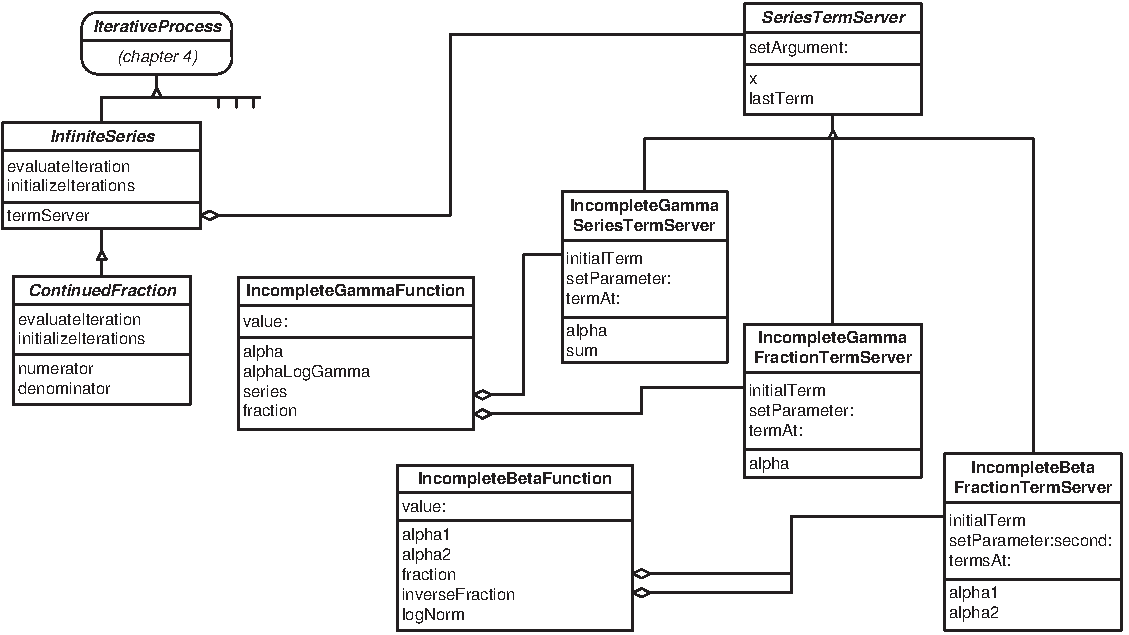
\includegraphics[width=11cm]{Figures/SeriesClassDiagram}
\caption{Smalltalk class diagram for infinite series and continued
fractions}\label{fig:StSeriesClass}
\end{figure}

The Smalltalk implementation uses two general-purpose classes to
implement an infinite series and a continued fraction
respectively. Each class then use a \patstyle{Strategy} pattern
class \cite{GoF} to compute each term of the expansion.

\section{Infinite series}
Many functions are defined with an infinite series, that is a sum
of an infinite number of terms. The most well known example is the
series for the exponential function:
\begin{equation}
  e^x=\sum_{n=0}^{\infty}{x^n \over n!}.
\end{equation}
For such a series to be defined, the terms of the series must
become very small as the index increases. If that is the case an
infinite series may be used to evaluate a function, for which no
closed expression exists. For this to be practical, however, the
series should converge quickly so that only a few terms are
needed. For example, computing the exponential of 6 to the
precision of an IEEE 32 bit floating number requires nearly 40
terms. This is clearly not an efficient way to compute the
exponential.

Discussing the convergence of a series is outside of the scope of
this book. Let us just state that in general numerical convergence
of a series is much harder to achieve than mathematical
convergence. In other words the fact that a series is defined
mathematically does not ensure that it can be evaluated
numerically.

A special remark pertains to alternating series. In an alternating
series the signs of consecutive terms are opposite. Trigonometric
functions have such a series expansion. Alternating series have
very bad numerical convergence properties: if the terms are large
rounding errors might suppress the convergence altogether. If one
cannot compute the function in another way it is best to compute
the terms of an alternating series in pairs to avoid rounding
errors.

In practice, a series must be tested for quick numerical
convergence prior to its implementation. As for rounding errors
the safest way is to do this experimentally, that is, print out
the terms of the series for a few representative\footnote{By {\sl
representative}, I mean either values, which are covering the
domain over which the function will be evaluated, or values, which
are suspected to give convergence problems.} values of the
variable. In the rest of this chapter we shall assume that this
essential step has been made.

To evaluate an infinite series, one carries the summation until
the last added term becomes smaller than the desired precision.
This kind of logic is quite similar to that of an iterative
process. Thus, the object used to compute an infinite series
belongs to a subclass of the iterative process classe discussed in
chapter \ref{ch:iteration}.

\subsection{Infinite series --- Smalltalk  implementation}
\label{sec:sseries}\marginpar{Figure \ref{fig:StSeriesClass} with
the boxes {\bf InfiniteSeries} and {\bf SeriesTermServer} grayed.}
Listing \ref{ls:infseries} shows a general Smalltalk
implementation of a class evaluating an infinite series. The class
being abstract, we do not give examples here. Concrete examples
are given in section \ref{sec:sincgamma}.

The Smalltalk implementation uses a \patstyle{Strategy} pattern.
The class {\tt DhbInfiniteSeries} is a subclass of the class {\tt
DhbIterativeProcess}, discussed in section \ref{sec:siteration}.
This class does not implement the algorithm needed to compute the
terms of the series directly. It delegates this responsibility to
an object stored in the instance variable {\tt termServer}. Two
hook methods, {\tt initialTerm} and {\tt termAt:} are used to
obtain the terms of the series from the term server object.

The method {\tt evaluateIteration} uses the method {\tt
precisionOf:relativeTo:} to return a relative precision as
discussed in section \ref{sec:siterrel}.

To implement a specific series, an object of the class {\tt
DhbInfiniteSeries} is instantiated with a specific term server. A
concrete example will be shown in section \ref{sec:sincgamma}.

Because of its generic nature, the class {\tt DhbInfiniteSeries}
does not implement the function behavior described in section
\ref{sec:stFunction} (method {\tt value:}). It is the
responsibility of each object combining an infinite series with a
specific term server to implement the function behavior. An
example is given in section \ref{sec:sincgamma}.
\begin{listing} Smalltalk implementation of an infinite series \label{ls:infseries}
$$\halign{ #\hfil&\quad#\hfil\cr {\sl Class}& {\Large\bf DhbInfiniteSeries}\cr
{\sl Subclass of }&{\tt DhbIterativeProcess}\cr\noalign{\vskip 1ex}

{\sl Instance variable names:}&\parbox[t]{4 in}{\tt  termServer }\cr\noalign{\vskip 1ex}}$$


Class methods
{\parskip 1ex\par\noindent}
{\bf server:} {\tt aTermServer}
\begin{verbatim}
    ^self new initialize: aTermServer
\end{verbatim}

Instance methods
{\parskip 1ex\par\noindent}
{\bf evaluateIteration}
\begin{verbatim}
    | delta |
    delta := termServer termAt: iterations.
    result := result + delta.
    ^ self precisionOf: delta abs relativeTo: result abs
\end{verbatim}
{\bf initialize:} {\tt aTermServer}
\begin{verbatim}
    termServer := aTermServer.
    ^ self
\end{verbatim}
{\bf initializeIterations}
\begin{verbatim}
    result := termServer initialTerm
\end{verbatim}


\end{listing}
The computation of the terms of the series is delegated to an
object instantiated from a server class. The abstract server class
is called {\tt DhbInfiniteSeriesTermServer}. It is responsible to
compute the terms at each iteration. This class receives the
argument of the function defined by the series, which is kept in
the instance variable {\tt x}. The instance variable {\tt
lastTerm} is provided to keep the last computed term since the
next term can often be computed from the previous one. The code of
this abstract class is shown in Listing 44.
\begin{listing} Smalltalk implementation of a term server \label{ls:termserver}
$$\halign{ #\hfil&\quad#\hfil\cr {\sl Class}& {\Large\bf DhbSeriesTermServer}\cr
{\sl Subclass of }&{\tt Object}\cr\noalign{\vskip 1ex}

{\sl Instance variable names:}&\parbox[t]{4 in}{\tt  x lastTerm }\cr\noalign{\vskip 1ex}}$$


Instance methods
{\parskip 1ex\par\noindent}
{\bf setArgument:} {\tt aNumber}
\begin{verbatim}
    x := aNumber asFloat.
\end{verbatim}


\end{listing}

\section{Continued fractions}
\label{sec:contfractions}
A continued fraction is an infinite
series of cascading fractions of the following form:
\begin{equation}
\label{eq:contfractions}
  f\left( x\right)=b_0+{a_1 \over\displaystyle b_1+
  {\strut a_2 \over\displaystyle b_2+{\strut a_3 \over\displaystyle b_3+
  {\strut a_4 \over\displaystyle b_4+\cdots}}}}
\end{equation}
In general, both sets of coefficients $a_0,\ldots$ and
$b_0,\ldots$ depend on the function's argument $x$. This
dependence in implicit in equation \ref{eq:contfractions} to keep
the notation simple. Since the above expression is quite awkward
to read - besides being a printer's nightmare - one usually uses a
linear notation as follows \cite{AbrSteg}, \cite{Press}:
\begin{equation}
\label{eq:contfractionsline}
  f\left( x\right)=b_0+{a_1 \over b_1+}{a_2 \over b_2+}{a_3 \over b_3+}{a_4 \over
  b_4+}\cdots
\end{equation}
The problem in evaluating such a fraction is that, {\it a priori},
one must begin the evaluation from the last term. Fortunately,
methods allowing the evaluation from the beginning of the
fractions have been around since the seventeen's century. A
detailed discussion of several methods is given in \cite{Press}.
In this book, we shall only discuss the modified Lentz' method
which has the advantage to work for a large class of fractions.

Implementing the other methods discussed in \cite{Press} is left
as an exercise to the reader. The corresponding classes can be
subclassed from the classes found in this chapter.

In 1976, Lentz proposed the following two auxiliary series:
\begin{equation}
  \left\{{
  \begin{array}{lcl}
    C_0 & = & b_0,\\
    D_0 & = & 0, \\
    C_n & = & {a_n \over C_{n-1}}+b_n\mbox{\quad for $n>0$}, \\
    D_n & = & {1 \over a_n D_{n-1}+b_n}\mbox{\quad for $n>0$}.
  \end{array}
  }\right.
\end{equation}
These two series are used to construct the series:
\begin{equation}
  \left\{{
  \begin{array}{lcl}
    f_0 & = & C_0,\\
    f_n & = & f_{n-1}C_n D_n. \\
  \end{array}
  }\right.
\end{equation}
One can prove by induction that this series converges toward the
continued fraction as $n$ gets large.

In general continued fractions have excellent convergence
properties. Some care, however, must be given when one of the
auxiliary terms $C_n$ or $1/D_n$ become nearly zero\footnote{That
is, a value which is zero within the precision of the numerical
representation.}. To avoid rounding errors, Thompson and Barnett,
in 1986, proposed a modification of the Lentz method in which any
value of the coefficients smaller than a small floor value is
adjusted to the floor value \cite{Press}. The floor value is
chosen to be the machine precision of the floating-point
representation (instance variable {\tt smallNumber} described in
section \ref{sec:findprecision}).

In terms of architecture, the implementation of a continued
fraction is similar to that of the infinite series.

\subsection{Continued fractions --- Smalltalk  implementation}
\marginpar{Figure \ref{fig:StSeriesClass} with the box {\bf
ContinuedFraction} grayed.} Listing \ref{ls:contfractions} shows
the implementation of a continued fraction in Smalltalk.

The class {\tt DhbContinuedFraction} is built as a subclass of the
class {\tt DhbInfiniteSeries}. Thus, it uses also the
\patstyle{Strategy} pattern.

The method {\tt limitedSmallValue:} implements the prescription of
Thompson and Barnett.
\begin{listing} Smalltalk implementation of a continued fraction \label{ls:contfractions}
$$\halign{ #\hfil&\quad#\hfil\cr {\sl Class}& {\Large\bf DhbContinuedFraction}\cr
{\sl Subclass of }&{\tt DhbInfiniteSeries}\cr\noalign{\vskip 1ex}

{\sl Instance variable names:}&\parbox[t]{4 in}{\tt  numerator denominator }\cr\noalign{\vskip 1ex}}$$


Instance methods
{\parskip 1ex\par\noindent}
{\bf evaluateIteration}
\begin{verbatim}
    | terms delta |
    terms := termServer termsAt: iterations.
    denominator := 1 / (self limitedSmallValue: ((terms at: 1) * denominator + (terms at: 2))).
    numerator := self limitedSmallValue: ((terms at: 1) / numerator + (terms at: 2)).
    delta := numerator * denominator.
    result := result * delta.
    ^ (delta - 1) abs
\end{verbatim}
{\bf initializeIterations}
\begin{verbatim}
    numerator := self limitedSmallValue: termServer initialTerm.
    denominator := 0.
    result := numerator
\end{verbatim}
{\bf limitedSmallValue:} {\tt aNumber}
\begin{verbatim}
    ^aNumber abs < DhbFloatingPointMachine new smallNumber
            ifTrue: [ DhbFloatingPointMachine new smallNumber ]
            ifFalse: [ aNumber ]
\end{verbatim}


\end{listing}

\section{Incomplete Gamma function}
\label{sec:incGamma} The incomplete gamma function is the integral
of a gamma distribution. It is used in statistics to evaluate the
probability of finding a measurement larger than a given value
when the measurements are distributed according to a gamma
distribution. In particular, the incomplete gamma function is used
to compute the confidence level of $\chi^2$ values when assessing
the validity of a parametric fit. Several examples of use of this
function will be introduced in chapters \ref{ch:statistics} and
\ref{ch:estimation}.

Figure \ref{fig:incGamma} shows the incomplete gamma function
(solid line) and its corresponding probability density function
(dotted line) for $\alpha=2.5$.
\begin{figure}
\centering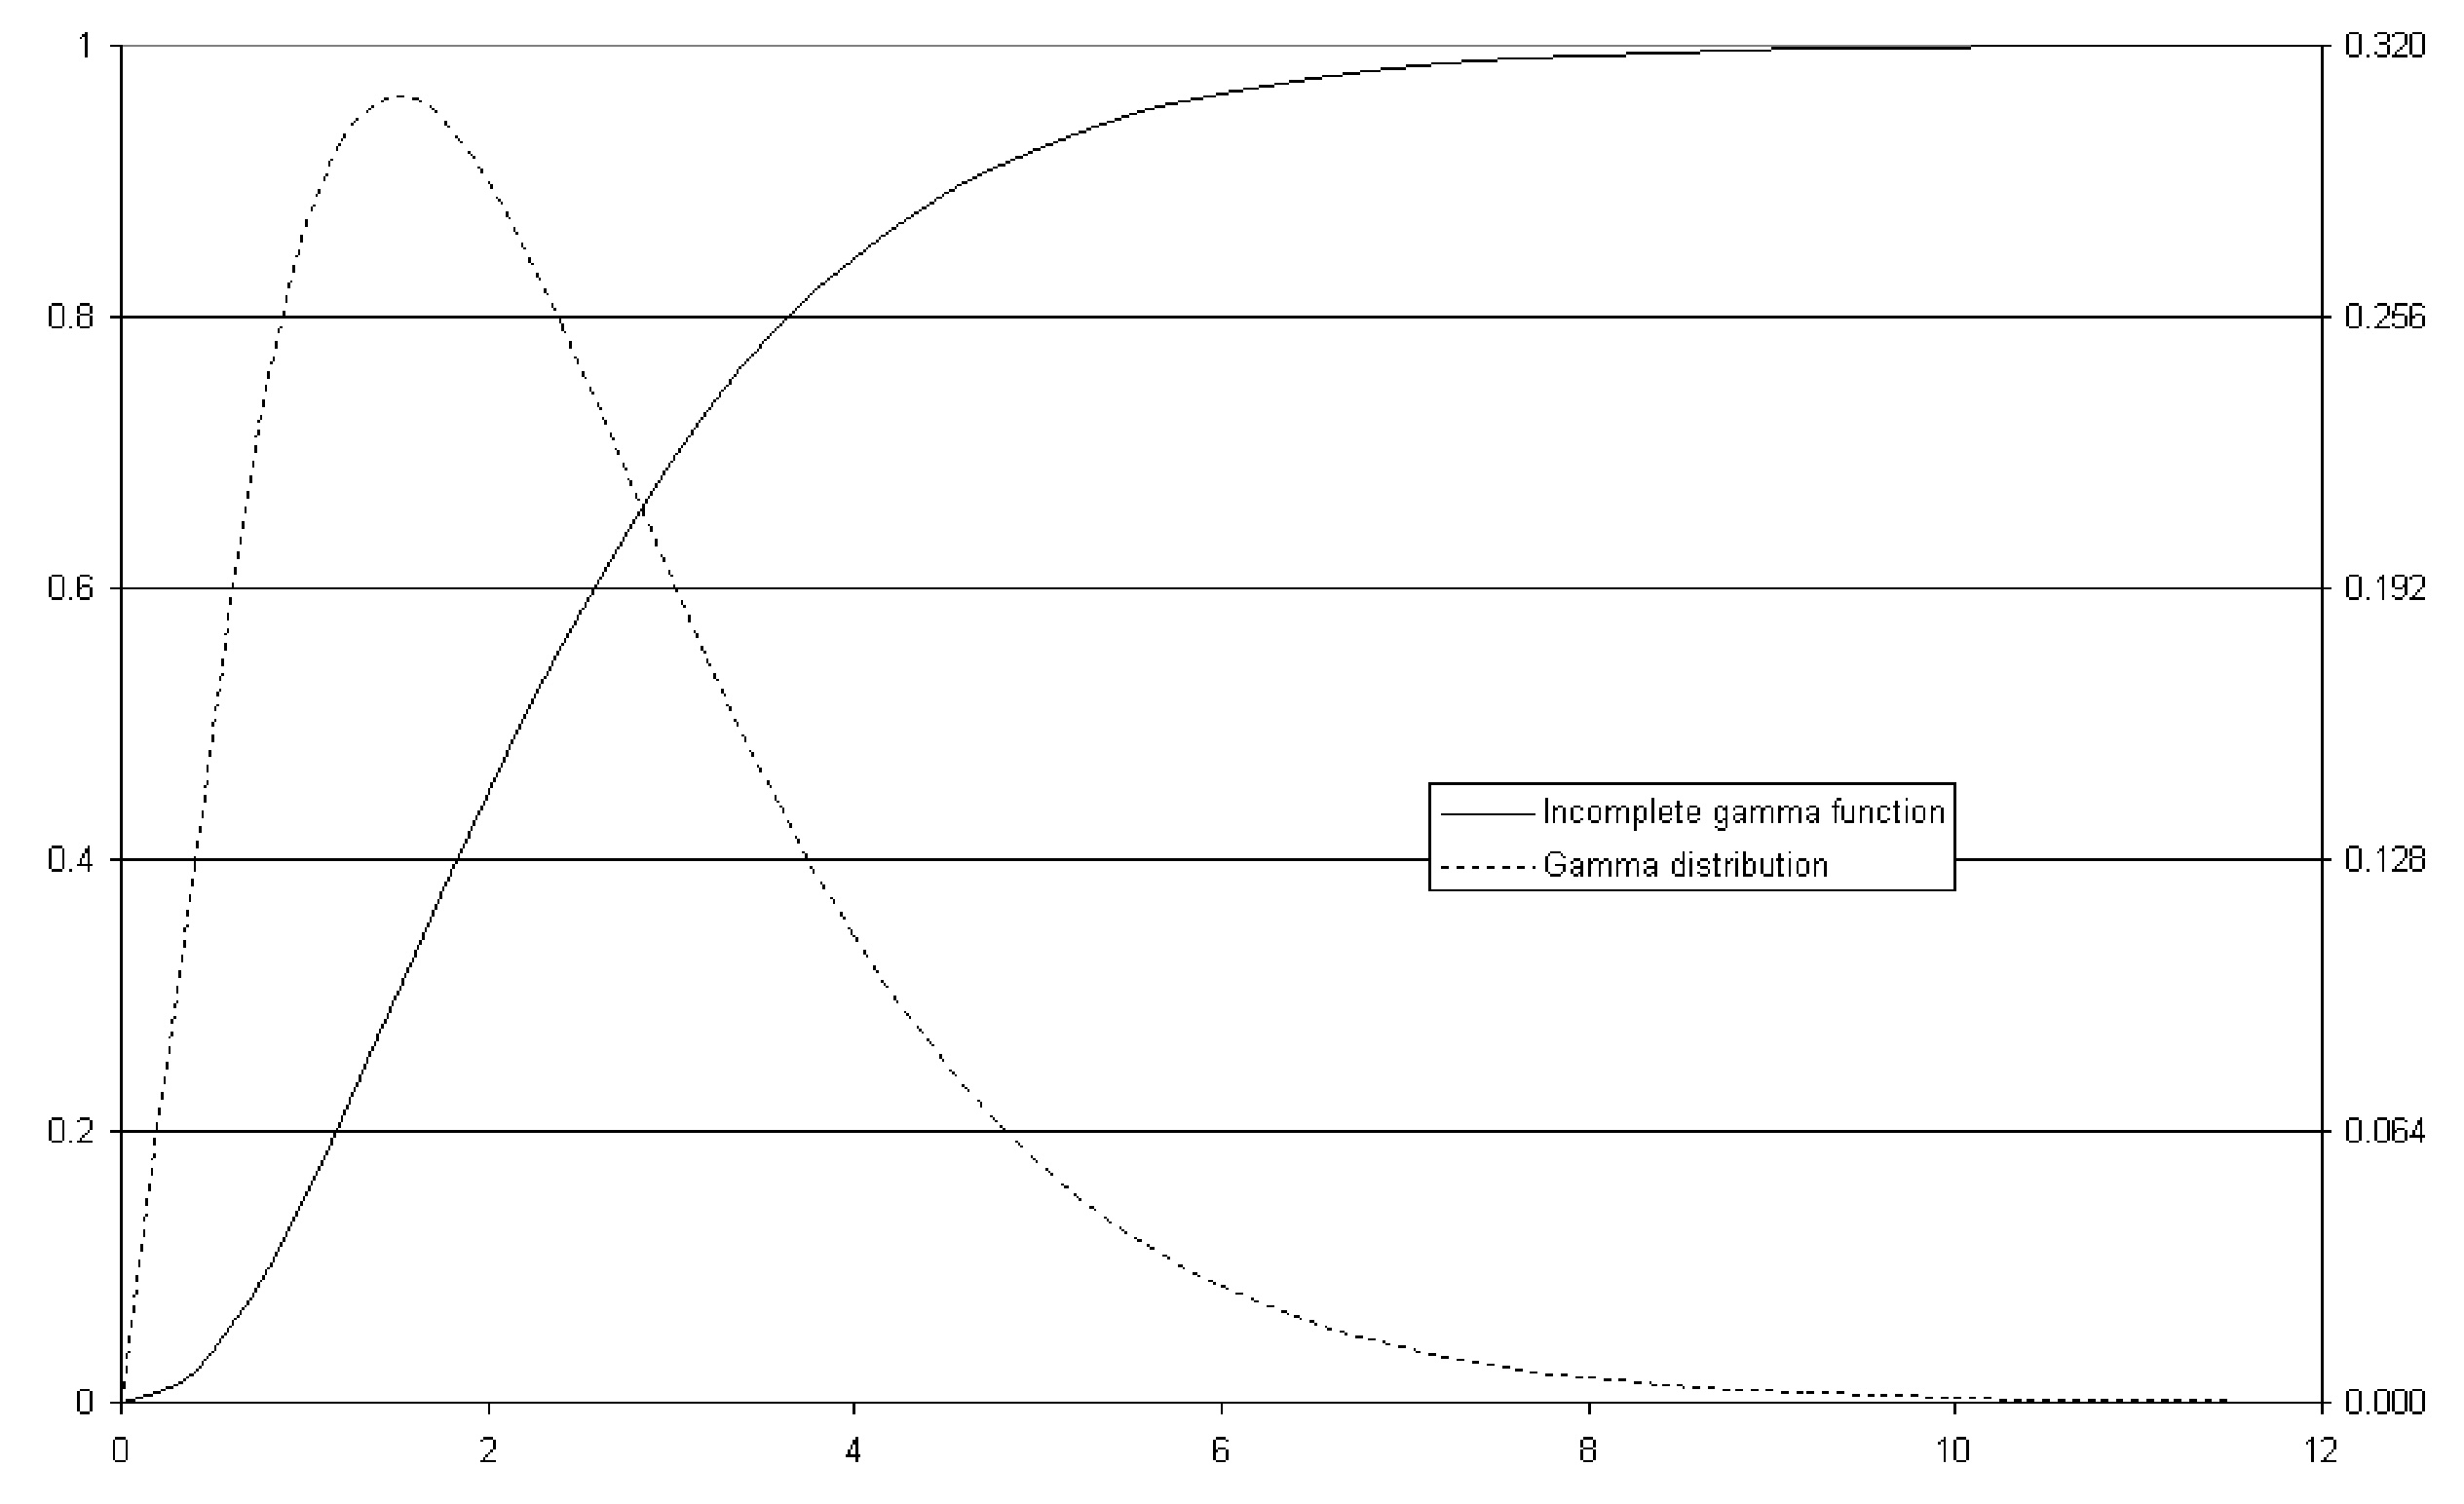
\includegraphics[width=10cm]{Figures/IncompleteGammaFunction}
\caption{The incomplete gamma function and the gamma distribution}\label{fig:incGamma}
\end{figure}

The gamma distribution is discussed in section
\ref{sec:gammadist}. The $\chi^2$ confidence level is discussed in
section \ref{sec:chitest}. General $\chi^2$ fits are discussed in
section \ref{sec:lsfnonlin}.

\subsection{Mathematical definitions}
\label{sec:incgamma} The incomplete gamma function is defined by
the following integral:
\begin{equation}
  \Gamma\left(x,\alpha\right)={1\over\Gamma\left(\alpha\right)}
  \int_0^x t^{\alpha -1} e^{-t} dt.
\end{equation}
Thus, the value of the incomplete gamma function lies between 0
and 1. The function has one parameter $\alpha$. The incomplete
gamma function is the distribution function of a gamma probability
density function with parameters $\alpha$ and 1 (\cf section
\ref{sec:gammadist} for a description of the gamma distribution
and its parameters). This integral can be expressed as the
following infinite series \cite{AbrSteg}:
\begin{equation}
\label{eq:incgammaser}
  \Gamma\left(x,\alpha\right)={e^{-x}x^\alpha\over\Gamma\left(\alpha\right)}
  \sum_{n=0}^{\infty}{\Gamma\left(\alpha\right) \over
  \Gamma\left(\alpha+1+n\right)}x^n.
\end{equation}
Written in this form we can see that each term of the series can
be computed from the previous one. Using the recurrence formula
for the gamma function --- equation \ref{eq:gammarec} in section
\ref{sec:gammafunc} --- we have:
\begin{mainEquation}
\label{eq:incgammaserterm}
  \left\{{
  \begin{array}{lcl}
    a_0 & = & {1\over\alpha},\\
    a_n & = & {x\over\alpha+1+n}a_{n-1}.
  \end{array}
  }\right.
\end{mainEquation}
The series in equation \ref{eq:incgammaser} converges well for
$x<\alpha+1$.

The incomplete gamma function can also be written as
\cite{AbrSteg}:
\begin{equation}
\label{eq:incgammafract}
  \Gamma\left(x,\alpha\right)={e^{-x}x^\alpha\over\Gamma\left(\alpha\right)}
  {1 \over F\left(x-\alpha+1,\alpha\right)},
\end{equation}
where $F\left(x,\alpha\right)$ is the continued fraction:
\begin{equation}
  F\left(x,\alpha\right)=x+{1\left(\alpha -1\right)\over x+2+}
  {2\left(\alpha -2\right)\over x+4+}
  {3\left(\alpha -3\right)\over x+6+}\ldots
\end{equation}
Using the notation introduced in equation
\ref{eq:contfractionsline} in section \ref{sec:contfractions} the
terms of the continued fraction are given by the following
expressions:
\begin{mainEquation}
\label{eq:incgammafractterm}
  \left\{{
  \begin{array}{lcl}
    b_n & = & x-\alpha+2n\mbox{\quad for $n=0,1,2,\ldots$}\\
    a_n & = &n\left(\alpha-n\right)\mbox{\quad for $n=1,2,\ldots$}
  \end{array}
  }\right.
\end{mainEquation}
It turns out that the continued fraction in equation
\ref{eq:incgammafract} converges for $x>\alpha+1$ \cite{Press},
that is, exactly where the series expansion of equation
\ref{eq:incgammaser} did not converge very well. Thus, the
incomplete gamma function can be computed using one of the two
methods depending on the range of the argument.

The reader will notice that equations \ref{eq:incgammaser} and
\ref{eq:incgammafract} have a common factor. The denominator of
that factor can be evaluated in advance in logarithmic form to
avoid floating-point overflow (\cf discussion in section
\ref{sec:gammafunc}). For each function evaluation the entire
factor is computed in logarithmic form to reduce rounding errors.
Then it is combined with the value of the series or the continued
fraction to compute the final result.

To avoid a floating-point error when evaluating the common factor,
the value of the incomplete gamma function at $x=0$ --- which is
of course 0 --- must be returned separately.

\subsection{Incomplete Gamma function --- Smalltalk  implementation}
\label{sec:sincgamma}\marginpar{Figure \ref{fig:StSeriesClass}
with the boxes {\bf IncompleteGammaFunction}, {\tt
IncompleteGammaSeriesTermServer} and {\tt
IncompleteGammaFractionTermServer} grayed.} Three classes are
needed to implement the incomplete gamma function in Smalltalk.
The class {\tt DhbIncompleteGamaFunction} is in charge of
computing the function itself. This is the object, which responds
to the method {\tt value:} to provide a function-like behavior to
the object. It is shown in Listing \ref{ls:incgamma} and has the
following instance variables.
\begin{description}
\item[\tt alpha]contains the function's parameter, \ie\ $\alpha$,
\item[\tt alphaLogGamma]used to cache the value of $\Gamma\left(\alpha\right)$ for efficiency
purposes,
\item[\tt series]contains the infinite series associated to the function,
\item[\tt fraction]contains the continued fraction  associated to the
function.
\end{description}
The instance variables {\tt series} and {\tt fraction} are
assigned using lazy initialization.

Depending on the range of the argument, the class delegates the
rest of the computing to either a series or a continued fraction.
In each case, a term server class provides the computation of the
terms. They are shown in listings \ref{ls:incgammasterm} and
\ref{ls:incgammafterm}.
\begin{listing} Smalltalk implementation of the incomplete gamma function \label{ls:incgamma}
$$\halign{ #\hfil&\quad#\hfil\cr {\sl Class}& {\Large\bf DhbIncompleteGammaFunction}\cr
{\sl Subclass of }&{\tt Object}\cr\noalign{\vskip 1ex}

{\sl Instance variable names:}&\parbox[t]{4 in}{\tt  alpha alphaLogGamma series fraction }\cr\noalign{\vskip 1ex}}$$


Class methods
{\parskip 1ex\par\noindent}
{\bf shape:} {\tt aNumber}
\begin{verbatim}
    ^super new initialize: aNumber
\end{verbatim}

Instance methods
{\parskip 1ex\par\noindent}
{\bf evaluateFraction:} {\tt aNumber}
\begin{verbatim}
    fraction isNil 
        ifTrue: 
            [fraction := DhbIncompleteGammaFractionTermServer new.
            fraction setParameter: alpha].
    fraction setArgument: aNumber.
    ^(DhbContinuedFraction server: fraction)
        desiredPrecision: DhbFloatingPointMachine new  defaultNumericalPrecision;
        evaluate
\end{verbatim}
{\bf evaluateSeries:} {\tt aNumber}
\begin{verbatim}
    series isNil
        ifTrue: [ series := DhbIncompleteGammaSeriesTermServer new.
                  series setParameter: alpha.
                ].
    series setArgument: aNumber.
    ^ (DhbInfiniteSeries server: series)
        desiredPrecision: DhbFloatingPointMachine new defaultNumericalPrecision;
        evaluate
\end{verbatim}
{\bf initialize:} {\tt aNumber}
\begin{verbatim}
    alpha := aNumber asFloat.
    alphaLogGamma := alpha logGamma.
    ^ self
\end{verbatim}
{\bf value:} {\tt aNumber}
\begin{verbatim}
    | x norm |
    aNumber = 0
        ifTrue: [ ^0].
    x := aNumber asFloat.
    norm := [ ( x ln * alpha - x - alphaLogGamma) exp] when: ExAll 
                                do: [ :signal | signal exitWith: nil ].
    norm isNil
        ifTrue: [ ^1].
    ^x - 1 < alpha
        ifTrue: [ ( self evaluateSeries: x) * norm ]
        ifFalse: [ 1 - ( norm / ( self evaluateFraction: x)) ]
\end{verbatim}


\end{listing}
Listing \ref{ls:incgammasterm} shows the implementation of the
term server for the series expansion. It needs two instance
variables: one to store the parameter $\alpha$; one to store the
sum accumulated in the denominator of equation
\ref{eq:incgammaserterm}. The two lines of equation
\ref{eq:incgammaserterm} are implemented respectively by the
methods {\tt initialTerm}  (for $n=0$) and {\tt termAt:} (for
$n\ge 1$).
\begin{listing} Smalltalk implementation of the series term server for the incomplete gamma function \label{ls:incgammasterm}
$$\halign{ #\hfil&\quad#\hfil\cr {\sl Class}& {\Large\bf DhbIncompleteGammaSeriesTermServer}\cr
{\sl Subclass of }&{\tt DhbSeriesTermServer}\cr\noalign{\vskip 1ex}

{\sl Instance variable names:}&\parbox[t]{4 in}{\tt  alpha sum }\cr\noalign{\vskip 1ex}}$$


Instance methods
{\parskip 1ex\par\noindent}
{\bf initialTerm}
\begin{verbatim}
    lastTerm := 1 / alpha.
    sum := alpha.
    ^lastTerm

\end{verbatim}
{\bf setParameter:} {\tt aNumber}
\begin{verbatim}
    alpha := aNumber asFloat

\end{verbatim}
{\bf termAt:} {\tt anInteger}
\begin{verbatim}
    sum := sum + 1.
    lastTerm := lastTerm * x / sum.
    ^lastTerm

\end{verbatim}


\end{listing}
Listing \ref{ls:incgammafterm} shows the implementation of the
term server for the continued fraction. It needs one instance
variable to store the parameter $\alpha$. Equation
\ref{eq:incgammafractterm} is implemented by the methods {\tt
initialTerm}  (for $n=0$) and {\tt termsAt:} (for $n\ge 1$).
\begin{listing} Smalltalk implementation of the fraction term server for the incomplete gamma function \label{ls:incgammafterm}
$$\halign{ #\hfil&\quad#\hfil\cr {\sl Class}& {\Large\bf DhbIncompleteGammaFractionTermServer}\cr
{\sl Subclass of }&{\tt DhbSeriesTermServer}\cr\noalign{\vskip 1ex}

{\sl Instance variable names:}&\parbox[t]{4 in}{\tt  alpha }\cr\noalign{\vskip 1ex}}$$


Instance methods
{\parskip 1ex\par\noindent}
{\bf initialTerm}
\begin{verbatim}
    lastTerm := x - alpha + 1.
    ^lastTerm

\end{verbatim}
{\bf setParameter:} {\tt aNumber}
\begin{verbatim}
    alpha := aNumber asFloat

\end{verbatim}
{\bf termsAt:} {\tt anInteger}
\begin{verbatim}
    lastTerm := lastTerm + 2.
    ^Array with: (alpha - anInteger) * anInteger with: lastTerm

\end{verbatim}


\end{listing}
An example of use of the incomplete gamma function can be found in
section \ref{sec:sgammadist}.


\section{Incomplete Beta function}
\label{sec:incbeta} The incomplete beta function is the integral
of a beta distribution. It used in statistics to evaluate the
probability of finding a measurement larger than a given value
when the measurements are distributed according to a beta
distribution. It is also used to compute the confidence level of
the Student distribution ($t$-test) and of the Fisher-Snedecor
distribution ($F$-test). The beta distribution is discussed in
section \ref{sec:betadist}. The $t$-test is discussed in section
\ref{sec:ttest}. The $F$-test is discussed in section
\ref{sec:Ftest}.

Figure \ref{fig:incBetaFunction} shows the incomplete beta
function (solid line) and its corresponding probability density
function (dotted line) for $\alpha_1=4.5$ and $\alpha_2=2.5$.
\begin{figure}
\centering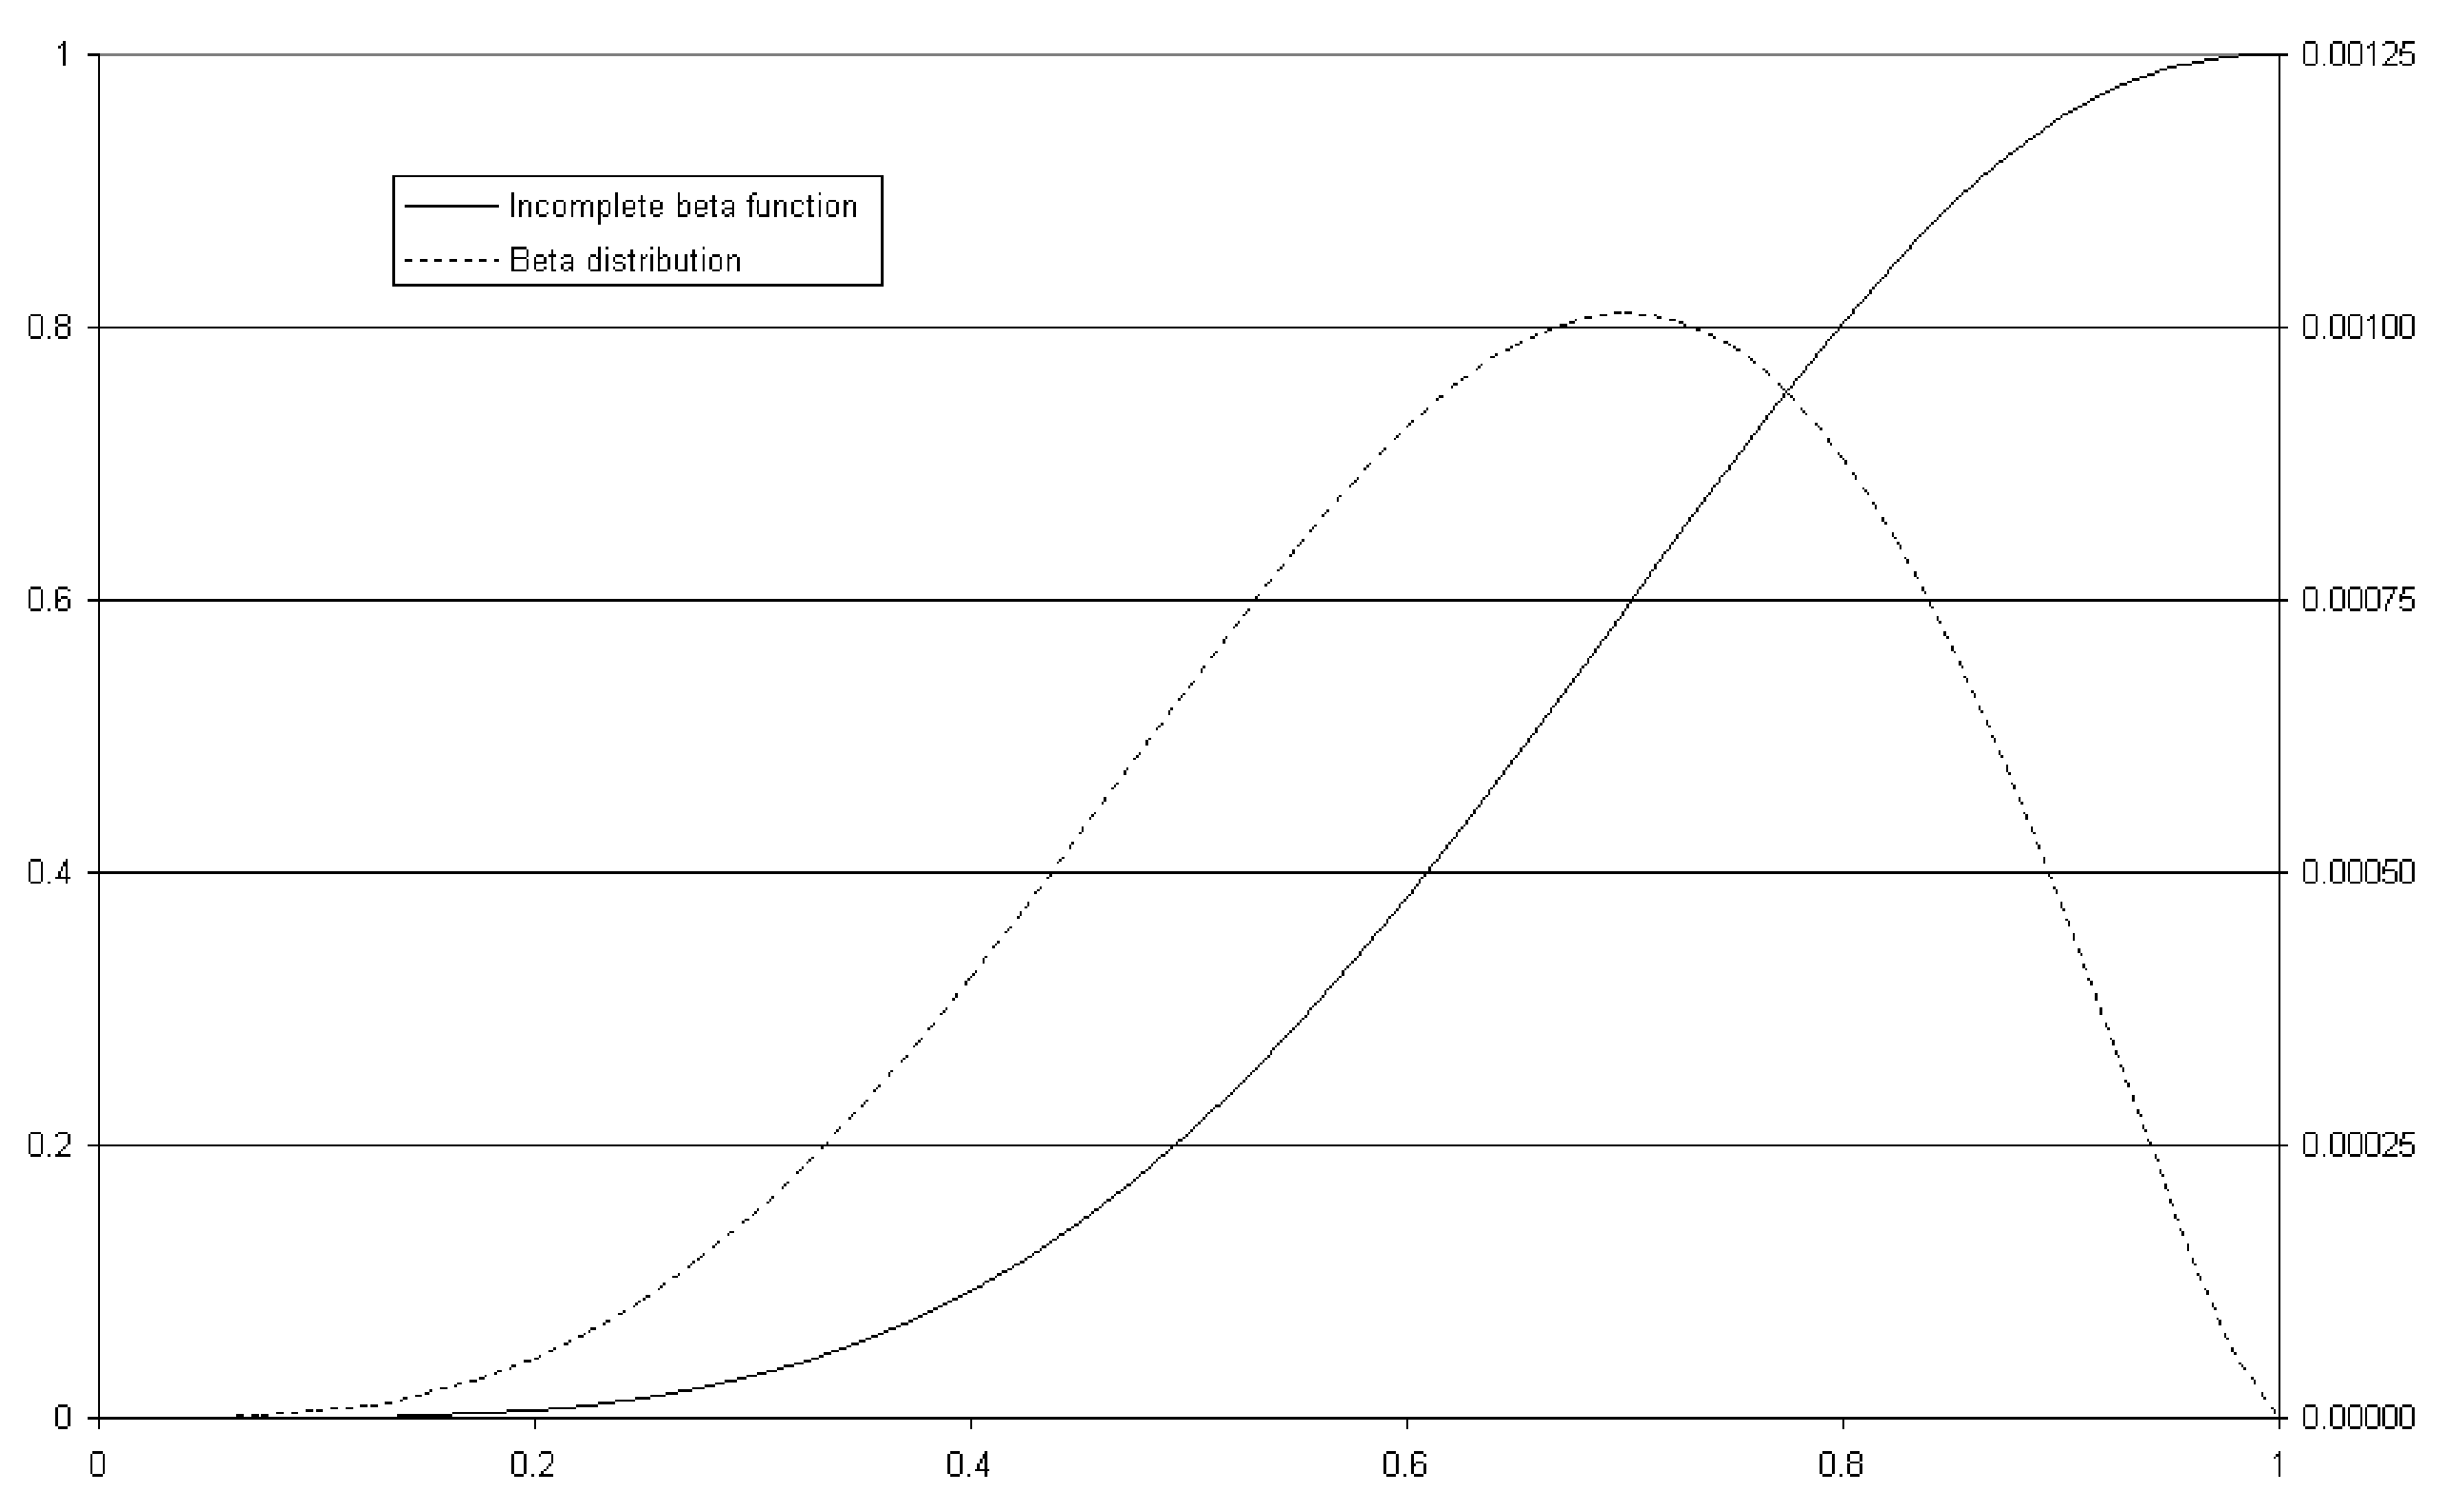
\includegraphics[width=10cm]{Figures/IncompleteBetaFunction}
\caption{The incomplete beta function and the beta distribution}\label{fig:incBetaFunction}
\end{figure}

\subsection{Mathematical definitions}
The incomplete beta function is defined over the interval
$\left[0,1\right]$ by the following integral:
\begin{equation}
\label{eq:incBetaFunction}
  B\left(x;\alpha_1,\alpha_2\right)={1\over B\left(\alpha_1,\alpha_2\right)}
  \int_0^x t^{\alpha_1-1}\left(1-t\right)^{\alpha_2-1}dt,
\end{equation}
where $B\left(\alpha_1,\alpha_2\right)$ is the beta function
defined in section \ref{sec:betafunc}. The function has two
parameters $\alpha_1$ and $\alpha_2$. By definition, the value of
the incomplete beta function is comprised between 0 and 1.

None of the series expansions of this integral have good numerical
convergence. There is, however, a continued fraction development
which converges over a sufficient range \cite{AbrSteg}:
\begin{equation}
\label{eq:incbeta}
  B\left(x;\alpha_1,\alpha_2\right)={x^{\alpha_1-1}\left(1-x\right)^{\alpha_2-1}\over
  \alpha_1 B\left(\alpha_1,\alpha_2\right)}
  {1\over F\left(x;\alpha_1,\alpha_2\right)},
\end{equation}
where
\begin{equation}
  F\left(x;\alpha_1,\alpha_2\right)=1+
  {a_1\over 1+}{a_2\over 1+}{a_3\over 1+}\cdots
\end{equation}
Using the notation introduced in section \ref{sec:contfractions}
we have:
\begin{mainEquation}
\label{eq:incbetaterm}
  \left\{{
  \begin{array}{lcl}
    b_n & = & 1\mbox{\quad for $n=0,1,2,\ldots$} \\*[1ex]
    a_{2n} & = & {\displaystyle n\left(\alpha_2-n\right)x \over \displaystyle\left(\alpha_1+2n\right)
    \left(\alpha_1+2n-1\right)} \mbox{\quad for $n=1,2,\ldots$} \\*[3ex]
    a_{2n+1} & = & {\displaystyle\left(\alpha_1+n\right)\left(\alpha_1+\alpha_2+n\right)x \over \displaystyle\left(\alpha_1+2n\right)
    \left(\alpha_1+2n-1\right)} \mbox{\quad for $n=1,2,\ldots$}
  \end{array}
  }\right.
\end{mainEquation}
The continued fraction in equation \ref{eq:incbeta} converges
rapidly for $x>{\alpha_1+1 \over
\alpha_1+\alpha_2+2}$\cite{Press}. To compute the incomplete beta
function over the complementary range, one uses the following
symmetry property of the function:
\begin{equation}
  B\left(x;\alpha_1,\alpha_2\right)=1-B\left(1-x;\alpha_2,\alpha_1\right)
\end{equation}
Since $1-x<{\alpha_2+1 \over \alpha_1+\alpha_2+2}$ if
$x<{\alpha_1+1 \over \alpha_1+\alpha_2+2}$, we can now compute the
function over the entire range.

To avoid a floating-point error when evaluating the leading factor
of equation \ref{eq:incbeta}, the values of the incomplete beta
function at $x=0$ --- which is 0 --- and at $x=1$ --- which is 1
--- must be returned separately.

\subsection{Incomplete Beta function --- Smalltalk  implementation}
\marginpar{Figure \ref{fig:StSeriesClass} with the boxes {\bf
IncompleteBetaFunction} and {\tt IncompleteBetaFractionTermServer}
grayed.} Listing \ref{ls:incbeta} shows the implementation of the
incomplete beta function in Smalltalk.

Two classes are needed to implement the incomplete beta function.
The class {\tt DhbIncompleteBetaFunction} is in charge of
computing the function itself. This class has the following
instance variables.
\begin{description}
\item[\tt alpha1]contains the first function's parameter, i.e.
$\alpha_1$,
\item[\tt alpha2]contains the second function's parameter, i.e.
$\alpha_2$,
\item[\tt logNorm]used to cache the value of $\ln B\left(\alpha_1,\alpha_2\right)$ for efficiency
purposes,
\item[\tt fraction]contains the continued fraction associated to the
function $B\left(x;\alpha_1,\alpha_2\right)$,
\item[\tt inverseFraction]contains the continued fraction associated to the
function $B\left(1-x;\alpha_2,\alpha_1\right)$.
\end{description}
Depending on the range of the argument, the class delegates the
rest of the computing to a continued fraction using the original
parameters or the reversed parameters if the symmetry relation
must be used. A term server class allows the computing of the
terms. Its code is shown in listing \ref{ls:incbetaterm}. The two
instance variables - {\tt fraction} and {\tt inverseFraction} -,
contain an instance of the term server, one for each permutation
of the parameters, thus preventing the unnecessary creation of new
instances of the term server at each evaluation. These instance
variables are assigned using lazy initialization.
\begin{listing} Smalltalk implementation of the incomplete beta function
\label{ls:incbeta}
$$\halign{ #\hfil&\quad#\hfil\cr {\sl Class}& {\Large\bf DhbIncompleteBetaFunction}\cr
{\sl Subclass of }&{\tt Object}\cr\noalign{\vskip 1ex}

{\sl Instance variable names:}&\parbox[t]{4 in}{\tt  alpha1 alpha2 fraction inverseFraction logNorm }\cr\noalign{\vskip 1ex}}$$


Class methods
{\parskip 1ex\par\noindent}
{\bf shape:} {\tt aNumber1} {\bf shape:} {\tt aNumber2}
\begin{verbatim}
    ^super new initialize: aNumber1 shape: aNumber2

\end{verbatim}



Instance methods
{\parskip 1ex\par\noindent}
{\bf evaluateFraction:} {\tt aNumber}
\begin{verbatim}
    fraction isNil 
        ifTrue: 
            [fraction := DhbIncompleteBetaFractionTermServer new.
            fraction setParameter: alpha1 second: alpha2].
    fraction setArgument: aNumber.
    ^(DhbContinuedFraction server: fraction)
        desiredPrecision: DhbFloatingPointMachine new 
                                            defaultNumericalPrecision;
        evaluate

\end{verbatim}
{\bf evaluateInverseFraction:} {\tt aNumber}
\begin{verbatim}
    inverseFraction isNil 
        ifTrue: 
            [inverseFraction := DhbIncompleteBetaFractionTermServer 
                                                                  new.
            inverseFraction setParameter: alpha2 second: alpha1].
    inverseFraction setArgument: (1 - aNumber).
    ^(DhbContinuedFraction server: inverseFraction)
        desiredPrecision: DhbFloatingPointMachine new 
                                            defaultNumericalPrecision;
        evaluate

\end{verbatim}
{\bf initialize:} {\tt aNumber1} {\bf shape:} {\tt aNumber2}
\begin{verbatim}
    alpha1 := aNumber1.
    alpha2 := aNumber2.
    logNorm := ( alpha1 + alpha2) logGamma - alpha1 logGamma - alpha2 
                                                             logGamma.
    ^self

\end{verbatim}
{\bf value:} {\tt aNumber}
\begin{verbatim}
    | norm |
    aNumber = 0
        ifTrue: [ ^0].
    aNumber = 1
        ifTrue: [ ^1].
    norm :=  ( aNumber ln * alpha1 + ( ( 1 - aNumber) ln * alpha2) + 
                                                         logNorm) exp.
    ^( alpha1 + alpha2 + 2) * aNumber < ( alpha1 + 1)
        ifTrue: [ norm / ( ( self evaluateFraction: aNumber) * 
                                                              alpha1)]
        ifFalse:[ 1 - ( norm / ( ( self evaluateInverseFraction: 
                                                  aNumber) * alpha2))]

\end{verbatim}


\end{listing}
Listing \ref{ls:incbetaterm} shows the implementation of the term
server. It needs two instance variables to store the parameters
$\alpha_1$ and $\alpha_2$. Equation \ref{eq:incbetaterm} is
implemented by the methods {\tt initialTerm} (for $n=0$) and {\tt
termsAt:} (for $n\ge 1$).
\begin{listing} Smalltalk implementation of the term server for the incomplete beta function
\label{ls:incbetaterm}
$$\halign{ #\hfil&\quad#\hfil\cr {\sl Class}& {\Large\bf DhbIncompleteBetaFractionTermServer}\cr
{\sl Subclass of }&{\tt DhbSeriesTermServer}\cr\noalign{\vskip 1ex}

{\sl Instance variable names:}&\parbox[t]{4 in}{\tt  alpha1 alpha2 }\cr\noalign{\vskip 1ex}}$$


Instance methods
{\parskip 1ex\par\noindent}
{\bf initialTerm}
\begin{verbatim}
    ^ 1
\end{verbatim}
{\bf setParameter:} {\tt aNumber1} {\bf second:} {\tt aNumber2}
\begin{verbatim}
    alpha1 := aNumber1.
    alpha2 := aNumber2
\end{verbatim}
{\bf termsAt:} {\tt anInteger}
\begin{verbatim}
    | n n2 |
    n := anInteger // 2.
    n2 := 2 * n.
    ^Array with: ( n2 < anInteger 
        ifTrue: [ x negated * (alpha1 + n) * (alpha1 + alpha2 + n) 
                                / ((alpha1 + n2) * (alpha1 + 1 + n2))]
        ifFalse: [x * n * (alpha2 - n) / ((alpha1 + n2) * (alpha1 - 1 + n2)) ])
            with: 1
\end{verbatim}


\end{listing}
An example of use of the incomplete beta function can be found in
sections \ref{sec:Ftest} and \ref{sec:ttest}.


\ifx\wholebook\relax\else\end{document}\fi
